\documentclass[1p]{elsarticle_modified}
%\bibliographystyle{elsarticle-num}

%\usepackage[colorlinks]{hyperref}
%\usepackage{abbrmath_seonhwa} %\Abb, \Ascr, \Acal ,\Abf, \Afrak
\usepackage{amsfonts}
\usepackage{amssymb}
\usepackage{amsmath}
\usepackage{amsthm}
\usepackage{scalefnt}
\usepackage{amsbsy}
\usepackage{kotex}
\usepackage{caption}
\usepackage{subfig}
\usepackage{color}
\usepackage{graphicx}
\usepackage{xcolor} %% white, black, red, green, blue, cyan, magenta, yellow
\usepackage{float}
\usepackage{setspace}
\usepackage{hyperref}

\usepackage{tikz}
\usetikzlibrary{arrows}

\usepackage{multirow}
\usepackage{array} % fixed length table
\usepackage{hhline}

%%%%%%%%%%%%%%%%%%%%%
\makeatletter
\renewcommand*\env@matrix[1][\arraystretch]{%
	\edef\arraystretch{#1}%
	\hskip -\arraycolsep
	\let\@ifnextchar\new@ifnextchar
	\array{*\c@MaxMatrixCols c}}
\makeatother %https://tex.stackexchange.com/questions/14071/how-can-i-increase-the-line-spacing-in-a-matrix
%%%%%%%%%%%%%%%

\usepackage[normalem]{ulem}

\newcommand{\msout}[1]{\ifmmode\text{\sout{\ensuremath{#1}}}\else\sout{#1}\fi}
%SOURCE: \msout is \stkout macro in https://tex.stackexchange.com/questions/20609/strikeout-in-math-mode

\newcommand{\cancel}[1]{
	\ifmmode
	{\color{red}\msout{#1}}
	\else
	{\color{red}\sout{#1}}
	\fi
}

\newcommand{\add}[1]{
	{\color{blue}\uwave{#1}}
}

\newcommand{\replace}[2]{
	\ifmmode
	{\color{red}\msout{#1}}{\color{blue}\uwave{#2}}
	\else
	{\color{red}\sout{#1}}{\color{blue}\uwave{#2}}
	\fi
}

\newcommand{\Sol}{\mathcal{S}} %segment
\newcommand{\D}{D} %diagram
\newcommand{\A}{\mathcal{A}} %arc


%%%%%%%%%%%%%%%%%%%%%%%%%%%%%5 test

\def\sl{\operatorname{\textup{SL}}(2,\Cbb)}
\def\psl{\operatorname{\textup{PSL}}(2,\Cbb)}
\def\quan{\mkern 1mu \triangleright \mkern 1mu}

\theoremstyle{definition}
\newtheorem{thm}{Theorem}[section]
\newtheorem{prop}[thm]{Proposition}
\newtheorem{lem}[thm]{Lemma}
\newtheorem{ques}[thm]{Question}
\newtheorem{cor}[thm]{Corollary}
\newtheorem{defn}[thm]{Definition}
\newtheorem{exam}[thm]{Example}
\newtheorem{rmk}[thm]{Remark}
\newtheorem{alg}[thm]{Algorithm}

\newcommand{\I}{\sqrt{-1}}
\begin{document}

%\begin{frontmatter}
%
%\title{Boundary parabolic representations of knots up to 8 crossings}
%
%%% Group authors per affiliation:
%\author{Yunhi Cho} 
%\address{Department of Mathematics, University of Seoul, Seoul, Korea}
%\ead{yhcho@uos.ac.kr}
%
%
%\author{Seonhwa Kim} %\fnref{s_kim}}
%\address{Center for Geometry and Physics, Institute for Basic Science, Pohang, 37673, Korea}
%\ead{ryeona17@ibs.re.kr}
%
%\author{Hyuk Kim}
%\address{Department of Mathematical Sciences, Seoul National University, Seoul 08826, Korea}
%\ead{hyukkim@snu.ac.kr}
%
%\author{Seokbeom Yoon}
%\address{Department of Mathematical Sciences, Seoul National University, Seoul, 08826,  Korea}
%\ead{sbyoon15@snu.ac.kr}
%
%\begin{abstract}
%We find all boundary parabolic representation of knots up to 8 crossings.
%
%\end{abstract}
%\begin{keyword}
%    \MSC[2010] 57M25 
%\end{keyword}
%
%\end{frontmatter}

%\linenumbers
%\tableofcontents
%
\newcommand\colored[1]{\textcolor{white}{\rule[-0.35ex]{0.8em}{1.4ex}}\kern-0.8em\color{red} #1}%
%\newcommand\colored[1]{\textcolor{white}{ #1}\kern-2.17ex	\textcolor{white}{ #1}\kern-1.81ex	\textcolor{white}{ #1}\kern-2.15ex\color{red}#1	}

{\Large $\underline{12n_{0213}~(K12n_{0213})}$}

\setlength{\tabcolsep}{10pt}
\renewcommand{\arraystretch}{1.6}
\vspace{1cm}\begin{tabular}{m{100pt}>{\centering\arraybackslash}m{274pt}}
\multirow{5}{120pt}{
	\centering
	\includegraphics[width=112pt]{../../../GIT/diagram.site/Diagrams/png/2302_12n_0213.png}\\
\ \ \ A knot diagram\footnotemark}&
\allowdisplaybreaks
\textbf{Linearized knot diagam} \\
\cline{2-2}
 &
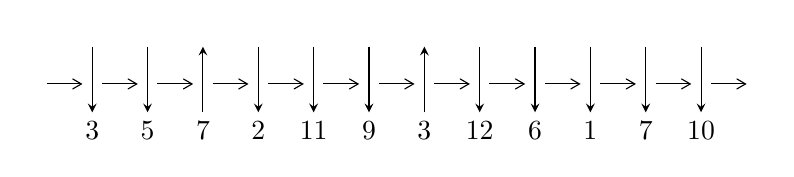
\begin{tikzpicture}[x=20pt, y=17pt]
	% nodes
	\node (C0) at (0, 0) {};
	\node (C1) at (1, 0) {};
	\node (C1U) at (1, +1) {};
	\node (C1D) at (1, -1) {3};

	\node (C2) at (2, 0) {};
	\node (C2U) at (2, +1) {};
	\node (C2D) at (2, -1) {5};

	\node (C3) at (3, 0) {};
	\node (C3U) at (3, +1) {};
	\node (C3D) at (3, -1) {7};

	\node (C4) at (4, 0) {};
	\node (C4U) at (4, +1) {};
	\node (C4D) at (4, -1) {2};

	\node (C5) at (5, 0) {};
	\node (C5U) at (5, +1) {};
	\node (C5D) at (5, -1) {11};

	\node (C6) at (6, 0) {};
	\node (C6U) at (6, +1) {};
	\node (C6D) at (6, -1) {9};

	\node (C7) at (7, 0) {};
	\node (C7U) at (7, +1) {};
	\node (C7D) at (7, -1) {3};

	\node (C8) at (8, 0) {};
	\node (C8U) at (8, +1) {};
	\node (C8D) at (8, -1) {12};

	\node (C9) at (9, 0) {};
	\node (C9U) at (9, +1) {};
	\node (C9D) at (9, -1) {6};

	\node (C10) at (10, 0) {};
	\node (C10U) at (10, +1) {};
	\node (C10D) at (10, -1) {1};

	\node (C11) at (11, 0) {};
	\node (C11U) at (11, +1) {};
	\node (C11D) at (11, -1) {7};

	\node (C12) at (12, 0) {};
	\node (C12U) at (12, +1) {};
	\node (C12D) at (12, -1) {10};
	\node (C13) at (13, 0) {};

	% arrows
	\draw[->,>={angle 60}]
	(C0) edge (C1) (C1) edge (C2) (C2) edge (C3) (C3) edge (C4) (C4) edge (C5) (C5) edge (C6) (C6) edge (C7) (C7) edge (C8) (C8) edge (C9) (C9) edge (C10) (C10) edge (C11) (C11) edge (C12) (C12) edge (C13) ;	\draw[->,>=stealth]
	(C1U) edge (C1D) (C2U) edge (C2D) (C3D) edge (C3U) (C4U) edge (C4D) (C5U) edge (C5D) (C6U) edge (C6D) (C7D) edge (C7U) (C8U) edge (C8D) (C9U) edge (C9D) (C10U) edge (C10D) (C11U) edge (C11D) (C12U) edge (C12D) ;
	\end{tikzpicture} \\
\hhline{~~} \\& 
\textbf{Solving Sequence} \\ \cline{2-2} 
 &
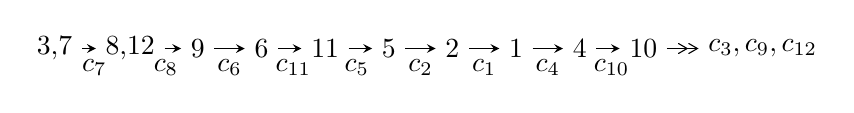
\begin{tikzpicture}[x=23pt, y=7pt]
	% node
	\node (A0) at (-1/8, 0) {3,7};
	\node (A1) at (17/16, 0) {8,12};
	\node (A2) at (17/8, 0) {9};
	\node (A3) at (25/8, 0) {6};
	\node (A4) at (33/8, 0) {11};
	\node (A5) at (41/8, 0) {5};
	\node (A6) at (49/8, 0) {2};
	\node (A7) at (57/8, 0) {1};
	\node (A8) at (65/8, 0) {4};
	\node (A9) at (73/8, 0) {10};
	\node (C1) at (1/2, -1) {$c_{7}$};
	\node (C2) at (13/8, -1) {$c_{8}$};
	\node (C3) at (21/8, -1) {$c_{6}$};
	\node (C4) at (29/8, -1) {$c_{11}$};
	\node (C5) at (37/8, -1) {$c_{5}$};
	\node (C6) at (45/8, -1) {$c_{2}$};
	\node (C7) at (53/8, -1) {$c_{1}$};
	\node (C8) at (61/8, -1) {$c_{4}$};
	\node (C9) at (69/8, -1) {$c_{10}$};
	\node (A10) at (11, 0) {$c_{3},c_{9},c_{12}$};

	% edge
	\draw[->,>=stealth]	
	(A0) edge (A1) (A1) edge (A2) (A2) edge (A3) (A3) edge (A4) (A4) edge (A5) (A5) edge (A6) (A6) edge (A7) (A7) edge (A8) (A8) edge (A9) ;
	\draw[->>,>={angle 60}]	
	(A9) edge (A10);
\end{tikzpicture} \\ 

\end{tabular} \\

\footnotetext{
The image of knot diagram is generated by the software ``\textbf{Draw programme}" developed by Andrew Bartholomew(\url{http://www.layer8.co.uk/maths/draw/index.htm\#Running-draw}), where we modified some parts for our purpose(\url{https://github.com/CATsTAILs/LinksPainter}).
}\phantom \\ \newline 
\centering \textbf{Ideals for irreducible components\footnotemark of $X_{\text{par}}$} 
 
\begin{align*}
I^u_{1}&=\langle 
-4.59949\times10^{269} u^{80}+6.86481\times10^{269} u^{79}+\cdots+5.51786\times10^{269} b+2.33003\times10^{272},\\
\phantom{I^u_{1}}&\phantom{= \langle  }-2.46814\times10^{269} u^{80}+3.35212\times10^{269} u^{79}+\cdots+1.10357\times10^{270} a+1.23485\times10^{272},\\
\phantom{I^u_{1}}&\phantom{= \langle  }u^{81}-2 u^{80}+\cdots+128 u+256\rangle \\
I^u_{2}&=\langle 
b,\;-9 u^4+4 u^3-3 u^2+17 a+18 u-1,\;u^5+u^4+2 u^3+u^2+u+1\rangle \\
\\
I^v_{1}&=\langle 
a,\;-941 v^7-2551 v^6-1791 v^5+6184 v^4+16309 v^3-15249 v^2+887 b-4192 v+1842,\\
\phantom{I^v_{1}}&\phantom{= \langle  }v^8+2 v^7-8 v^5-13 v^4+28 v^3-7 v^2-3 v+1\rangle \\
\end{align*}
\raggedright * 3 irreducible components of $\dim_{\mathbb{C}}=0$, with total 94 representations.\\
\footnotetext{All coefficients of polynomials are rational numbers. But the coefficients are sometimes approximated in decimal forms when there is not enough margin.}
\newpage
\renewcommand{\arraystretch}{1}
\centering \section*{I. $I^u_{1}= \langle -4.60\times10^{269} u^{80}+6.86\times10^{269} u^{79}+\cdots+5.52\times10^{269} b+2.33\times10^{272},\;-2.47\times10^{269} u^{80}+3.35\times10^{269} u^{79}+\cdots+1.10\times10^{270} a+1.23\times10^{272},\;u^{81}-2 u^{80}+\cdots+128 u+256 \rangle$}
\flushleft \textbf{(i) Arc colorings}\\
\begin{tabular}{m{7pt} m{180pt} m{7pt} m{180pt} }
\flushright $a_{3}=$&$\begin{pmatrix}0\\u\end{pmatrix}$ \\
\flushright $a_{7}=$&$\begin{pmatrix}1\\0\end{pmatrix}$ \\
\flushright $a_{8}=$&$\begin{pmatrix}1\\- u^2\end{pmatrix}$ \\
\flushright $a_{12}=$&$\begin{pmatrix}0.223650 u^{80}-0.303752 u^{79}+\cdots-220.646 u-111.896\\0.833564 u^{80}-1.24411 u^{79}+\cdots-1041.50 u-422.270\end{pmatrix}$ \\
\flushright $a_{9}=$&$\begin{pmatrix}0.0640486 u^{80}-0.0983033 u^{79}+\cdots-107.977 u-39.3161\\-0.588758 u^{80}+0.829945 u^{79}+\cdots+564.671 u+265.326\end{pmatrix}$ \\
\flushright $a_{6}=$&$\begin{pmatrix}-0.0674337 u^{80}+0.135096 u^{79}+\cdots+187.141 u+50.7879\\0.563979 u^{80}-0.802383 u^{79}+\cdots-556.962 u-256.795\end{pmatrix}$ \\
\flushright $a_{11}=$&$\begin{pmatrix}1.05721 u^{80}-1.54786 u^{79}+\cdots-1262.14 u-534.166\\0.833564 u^{80}-1.24411 u^{79}+\cdots-1041.50 u-422.270\end{pmatrix}$ \\
\flushright $a_{5}=$&$\begin{pmatrix}0.314943 u^{80}-0.447399 u^{79}+\cdots-386.680 u-179.586\\0.697460 u^{80}-1.02573 u^{79}+\cdots-848.797 u-360.306\end{pmatrix}$ \\
\flushright $a_{2}=$&$\begin{pmatrix}0.382518 u^{80}-0.578331 u^{79}+\cdots-462.117 u-180.720\\0.697460 u^{80}-1.02573 u^{79}+\cdots-848.797 u-360.306\end{pmatrix}$ \\
\flushright $a_{1}=$&$\begin{pmatrix}0.382518 u^{80}-0.578331 u^{79}+\cdots-462.117 u-180.720\\0.598651 u^{80}-0.876596 u^{79}+\cdots-726.974 u-312.510\end{pmatrix}$ \\
\flushright $a_{4}=$&$\begin{pmatrix}u\\u\end{pmatrix}$ \\
\flushright $a_{10}=$&$\begin{pmatrix}0.412932 u^{80}-0.594022 u^{79}+\cdots-454.675 u-197.166\\-0.598651 u^{80}+0.876596 u^{79}+\cdots+726.974 u+312.510\end{pmatrix}$\\&\end{tabular}
\flushleft \textbf{(ii) Obstruction class $= -1$}\\~\\
\flushleft \textbf{(iii) Cusp Shapes $= -1.57477 u^{80}+2.25832 u^{79}+\cdots+1490.53 u+646.531$}\\~\\
\newpage\renewcommand{\arraystretch}{1}
\flushleft \textbf{(iv) u-Polynomials at the component}\newline \\
\begin{tabular}{m{50pt}|m{274pt}}
Crossings & \hspace{64pt}u-Polynomials at each crossing \\
\hline $$\begin{aligned}c_{1}\end{aligned}$$&$\begin{aligned}
&u^{81}+36 u^{80}+\cdots+29 u+1
\end{aligned}$\\
\hline $$\begin{aligned}c_{2},c_{4}\end{aligned}$$&$\begin{aligned}
&u^{81}-10 u^{80}+\cdots-13 u+1
\end{aligned}$\\
\hline $$\begin{aligned}c_{3},c_{7}\end{aligned}$$&$\begin{aligned}
&u^{81}-2 u^{80}+\cdots+128 u+256
\end{aligned}$\\
\hline $$\begin{aligned}c_{5}\end{aligned}$$&$\begin{aligned}
&17(17 u^{81}-14 u^{80}+\cdots-259698 u+23437)
\end{aligned}$\\
\hline $$\begin{aligned}c_{6},c_{9}\end{aligned}$$&$\begin{aligned}
&u^{81}-3 u^{80}+\cdots+3 u-1
\end{aligned}$\\
\hline $$\begin{aligned}c_{8}\end{aligned}$$&$\begin{aligned}
&17(17 u^{81}-148 u^{80}+\cdots-626508 u-174339)
\end{aligned}$\\
\hline $$\begin{aligned}c_{10},c_{12}\end{aligned}$$&$\begin{aligned}
&u^{81}-7 u^{80}+\cdots+339 u-289
\end{aligned}$\\
\hline $$\begin{aligned}c_{11}\end{aligned}$$&$\begin{aligned}
&u^{81}-2 u^{80}+\cdots-32096 u+9248
\end{aligned}$\\
\hline
\end{tabular}\\~\\
\newpage\renewcommand{\arraystretch}{1}
\flushleft \textbf{(v) Riley Polynomials at the component}\newline \\
\begin{tabular}{m{50pt}|m{274pt}}
Crossings & \hspace{64pt}Riley Polynomials at each crossing \\
\hline $$\begin{aligned}c_{1}\end{aligned}$$&$\begin{aligned}
&y^{81}+28 y^{80}+\cdots+6913 y-1
\end{aligned}$\\
\hline $$\begin{aligned}c_{2},c_{4}\end{aligned}$$&$\begin{aligned}
&y^{81}-36 y^{80}+\cdots+29 y-1
\end{aligned}$\\
\hline $$\begin{aligned}c_{3},c_{7}\end{aligned}$$&$\begin{aligned}
&y^{81}-48 y^{80}+\cdots+2080768 y-65536
\end{aligned}$\\
\hline $$\begin{aligned}c_{5}\end{aligned}$$&$\begin{aligned}
&289(289 y^{81}+19082 y^{80}+\cdots-6.59115\times10^{9} y-5.49293\times10^{8})
\end{aligned}$\\
\hline $$\begin{aligned}c_{6},c_{9}\end{aligned}$$&$\begin{aligned}
&y^{81}+45 y^{80}+\cdots+5 y-1
\end{aligned}$\\
\hline $$\begin{aligned}c_{8}\end{aligned}$$&$\begin{aligned}
&289(289 y^{81}-4428 y^{80}+\cdots-1.69694\times10^{11} y-3.03941\times10^{10})
\end{aligned}$\\
\hline $$\begin{aligned}c_{10},c_{12}\end{aligned}$$&$\begin{aligned}
&y^{81}-43 y^{80}+\cdots+4014687 y-83521
\end{aligned}$\\
\hline $$\begin{aligned}c_{11}\end{aligned}$$&$\begin{aligned}
&y^{81}+30 y^{80}+\cdots-1164952064 y-85525504
\end{aligned}$\\
\hline
\end{tabular}\\~\\
\newpage\flushleft \textbf{(vi) Complex Volumes and Cusp Shapes}
$$\begin{array}{c|c|c}  
\text{Solutions to }I^u_{1}& \I (\text{vol} + \sqrt{-1}CS) & \text{Cusp shape}\\
 \hline 
\begin{aligned}
u &= \phantom{-}0.917288 + 0.136182 I \\
a &= -1.80406 - 1.65669 I \\
b &= \phantom{-}0.466096 + 1.065420 I\end{aligned}
 & \phantom{-}1.75099 - 2.26560 I & \phantom{-0.000000 } 0 \\ \hline\begin{aligned}
u &= \phantom{-}0.917288 - 0.136182 I \\
a &= -1.80406 + 1.65669 I \\
b &= \phantom{-}0.466096 - 1.065420 I\end{aligned}
 & \phantom{-}1.75099 + 2.26560 I & \phantom{-0.000000 } 0 \\ \hline\begin{aligned}
u &= \phantom{-}0.120668 + 1.075100 I \\
a &= \phantom{-}0.110583 - 0.334996 I \\
b &= -0.63907 - 1.32827 I\end{aligned}
 & \phantom{-}3.50365 - 4.45577 I & \phantom{-0.000000 } 0 \\ \hline\begin{aligned}
u &= \phantom{-}0.120668 - 1.075100 I \\
a &= \phantom{-}0.110583 + 0.334996 I \\
b &= -0.63907 + 1.32827 I\end{aligned}
 & \phantom{-}3.50365 + 4.45577 I & \phantom{-0.000000 } 0 \\ \hline\begin{aligned}
u &= -1.065120 + 0.201662 I \\
a &= \phantom{-}0.13685 - 1.63080 I \\
b &= \phantom{-}0.90356 + 1.59497 I\end{aligned}
 & -0.801342 - 0.587804 I & \phantom{-0.000000 } 0 \\ \hline\begin{aligned}
u &= -1.065120 - 0.201662 I \\
a &= \phantom{-}0.13685 + 1.63080 I \\
b &= \phantom{-}0.90356 - 1.59497 I\end{aligned}
 & -0.801342 + 0.587804 I & \phantom{-0.000000 } 0 \\ \hline\begin{aligned}
u &= \phantom{-}1.102270 + 0.086046 I \\
a &= \phantom{-}0.731098 + 0.138738 I \\
b &= -1.77507 + 0.10621 I\end{aligned}
 & \phantom{-}2.29933 + 2.90155 I & \phantom{-0.000000 } 0 \\ \hline\begin{aligned}
u &= \phantom{-}1.102270 - 0.086046 I \\
a &= \phantom{-}0.731098 - 0.138738 I \\
b &= -1.77507 - 0.10621 I\end{aligned}
 & \phantom{-}2.29933 - 2.90155 I & \phantom{-0.000000 } 0 \\ \hline\begin{aligned}
u &= \phantom{-}0.377849 + 1.055930 I \\
a &= -0.042987 + 0.341087 I \\
b &= -0.154093 + 1.058040 I\end{aligned}
 & \phantom{-}2.93287 - 0.15502 I & \phantom{-0.000000 } 0 \\ \hline\begin{aligned}
u &= \phantom{-}0.377849 - 1.055930 I \\
a &= -0.042987 - 0.341087 I \\
b &= -0.154093 - 1.058040 I\end{aligned}
 & \phantom{-}2.93287 + 0.15502 I & \phantom{-0.000000 } 0\\
 \hline 
 \end{array}$$\newpage$$\begin{array}{c|c|c}  
\text{Solutions to }I^u_{1}& \I (\text{vol} + \sqrt{-1}CS) & \text{Cusp shape}\\
 \hline 
\begin{aligned}
u &= -1.124380 + 0.061386 I \\
a &= \phantom{-}0.045693 - 0.667032 I \\
b &= \phantom{-}1.263870 + 0.473188 I\end{aligned}
 & \phantom{-}0.245536 - 0.603566 I & \phantom{-0.000000 } 0 \\ \hline\begin{aligned}
u &= -1.124380 - 0.061386 I \\
a &= \phantom{-}0.045693 + 0.667032 I \\
b &= \phantom{-}1.263870 - 0.473188 I\end{aligned}
 & \phantom{-}0.245536 + 0.603566 I & \phantom{-0.000000 } 0 \\ \hline\begin{aligned}
u &= \phantom{-}1.109070 + 0.299410 I \\
a &= -0.44786 - 1.55704 I \\
b &= \phantom{-}0.27630 + 1.76877 I\end{aligned}
 & -1.06769 + 4.07791 I & \phantom{-0.000000 } 0 \\ \hline\begin{aligned}
u &= \phantom{-}1.109070 - 0.299410 I \\
a &= -0.44786 + 1.55704 I \\
b &= \phantom{-}0.27630 - 1.76877 I\end{aligned}
 & -1.06769 - 4.07791 I & \phantom{-0.000000 } 0 \\ \hline\begin{aligned}
u &= -0.304908 + 0.772829 I \\
a &= \phantom{-}1.70493 - 1.90308 I \\
b &= \phantom{-}1.263410 + 0.370125 I\end{aligned}
 & -1.76648 + 3.44608 I & -11.81203 - 6.71131 I \\ \hline\begin{aligned}
u &= -0.304908 - 0.772829 I \\
a &= \phantom{-}1.70493 + 1.90308 I \\
b &= \phantom{-}1.263410 - 0.370125 I\end{aligned}
 & -1.76648 - 3.44608 I & -11.81203 + 6.71131 I \\ \hline\begin{aligned}
u &= \phantom{-}0.037140 + 0.801194 I \\
a &= \phantom{-}0.424195 + 0.072722 I \\
b &= \phantom{-}0.321351 - 0.451413 I\end{aligned}
 & -0.644523 + 1.154210 I & -7.22358 - 5.30161 I \\ \hline\begin{aligned}
u &= \phantom{-}0.037140 - 0.801194 I \\
a &= \phantom{-}0.424195 - 0.072722 I \\
b &= \phantom{-}0.321351 + 0.451413 I\end{aligned}
 & -0.644523 - 1.154210 I & -7.22358 + 5.30161 I \\ \hline\begin{aligned}
u &= \phantom{-}1.181860 + 0.365384 I \\
a &= -0.322573 - 0.695076 I \\
b &= \phantom{-}1.16061 + 1.01997 I\end{aligned}
 & -0.44702 + 4.44359 I & \phantom{-0.000000 } 0 \\ \hline\begin{aligned}
u &= \phantom{-}1.181860 - 0.365384 I \\
a &= -0.322573 + 0.695076 I \\
b &= \phantom{-}1.16061 - 1.01997 I\end{aligned}
 & -0.44702 - 4.44359 I & \phantom{-0.000000 } 0\\
 \hline 
 \end{array}$$\newpage$$\begin{array}{c|c|c}  
\text{Solutions to }I^u_{1}& \I (\text{vol} + \sqrt{-1}CS) & \text{Cusp shape}\\
 \hline 
\begin{aligned}
u &= \phantom{-}0.305807 + 1.214000 I \\
a &= \phantom{-}0.138866 + 0.073449 I \\
b &= -0.076313 - 0.714540 I\end{aligned}
 & -1.00073 + 1.10337 I & \phantom{-0.000000 } 0 \\ \hline\begin{aligned}
u &= \phantom{-}0.305807 - 1.214000 I \\
a &= \phantom{-}0.138866 - 0.073449 I \\
b &= -0.076313 + 0.714540 I\end{aligned}
 & -1.00073 - 1.10337 I & \phantom{-0.000000 } 0 \\ \hline\begin{aligned}
u &= \phantom{-}1.259720 + 0.183479 I \\
a &= \phantom{-}0.42270 - 1.68355 I \\
b &= -0.647775 + 1.125350 I\end{aligned}
 & -0.57249 + 7.40525 I & \phantom{-0.000000 } 0 \\ \hline\begin{aligned}
u &= \phantom{-}1.259720 - 0.183479 I \\
a &= \phantom{-}0.42270 + 1.68355 I \\
b &= -0.647775 - 1.125350 I\end{aligned}
 & -0.57249 - 7.40525 I & \phantom{-0.000000 } 0 \\ \hline\begin{aligned}
u &= \phantom{-}1.271440 + 0.091622 I \\
a &= -1.26707 + 0.81502 I \\
b &= -0.635645 + 0.052930 I\end{aligned}
 & \phantom{-}3.70065 + 2.46096 I & \phantom{-0.000000 } 0 \\ \hline\begin{aligned}
u &= \phantom{-}1.271440 - 0.091622 I \\
a &= -1.26707 - 0.81502 I \\
b &= -0.635645 - 0.052930 I\end{aligned}
 & \phantom{-}3.70065 - 2.46096 I & \phantom{-0.000000 } 0 \\ \hline\begin{aligned}
u &= -1.207870 + 0.444621 I \\
a &= \phantom{-}0.756760 + 0.229343 I \\
b &= -2.00837 + 0.41189 I\end{aligned}
 & \phantom{-}1.14509 - 8.06770 I & \phantom{-0.000000 } 0 \\ \hline\begin{aligned}
u &= -1.207870 - 0.444621 I \\
a &= \phantom{-}0.756760 - 0.229343 I \\
b &= -2.00837 - 0.41189 I\end{aligned}
 & \phantom{-}1.14509 + 8.06770 I & \phantom{-0.000000 } 0 \\ \hline\begin{aligned}
u &= -0.031998 + 0.705333 I \\
a &= \phantom{-}2.25763 + 3.03351 I \\
b &= \phantom{-}0.595287 - 0.236308 I\end{aligned}
 & -0.856013 - 0.572838 I & -9.77883 - 6.76958 I \\ \hline\begin{aligned}
u &= -0.031998 - 0.705333 I \\
a &= \phantom{-}2.25763 - 3.03351 I \\
b &= \phantom{-}0.595287 + 0.236308 I\end{aligned}
 & -0.856013 + 0.572838 I & -9.77883 + 6.76958 I\\
 \hline 
 \end{array}$$\newpage$$\begin{array}{c|c|c}  
\text{Solutions to }I^u_{1}& \I (\text{vol} + \sqrt{-1}CS) & \text{Cusp shape}\\
 \hline 
\begin{aligned}
u &= -1.254380 + 0.379088 I \\
a &= \phantom{-}0.073419 - 0.993964 I \\
b &= \phantom{-}0.322122 + 0.778979 I\end{aligned}
 & -3.62852 - 1.44404 I & \phantom{-0.000000 } 0 \\ \hline\begin{aligned}
u &= -1.254380 - 0.379088 I \\
a &= \phantom{-}0.073419 + 0.993964 I \\
b &= \phantom{-}0.322122 - 0.778979 I\end{aligned}
 & -3.62852 + 1.44404 I & \phantom{-0.000000 } 0 \\ \hline\begin{aligned}
u &= -1.290060 + 0.297853 I \\
a &= -2.40362 + 0.15222 I \\
b &= -0.496430 + 0.171022 I\end{aligned}
 & \phantom{-}3.27537 - 3.11183 I & \phantom{-0.000000 } 0 \\ \hline\begin{aligned}
u &= -1.290060 - 0.297853 I \\
a &= -2.40362 - 0.15222 I \\
b &= -0.496430 - 0.171022 I\end{aligned}
 & \phantom{-}3.27537 + 3.11183 I & \phantom{-0.000000 } 0 \\ \hline\begin{aligned}
u &= -0.430170 + 1.261980 I \\
a &= \phantom{-}0.0208238 - 0.0730675 I \\
b &= \phantom{-}0.075154 + 0.342675 I\end{aligned}
 & -7.39266 - 4.46618 I & \phantom{-0.000000 } 0 \\ \hline\begin{aligned}
u &= -0.430170 - 1.261980 I \\
a &= \phantom{-}0.0208238 + 0.0730675 I \\
b &= \phantom{-}0.075154 - 0.342675 I\end{aligned}
 & -7.39266 + 4.46618 I & \phantom{-0.000000 } 0 \\ \hline\begin{aligned}
u &= \phantom{-}0.003874 + 1.341760 I \\
a &= -0.051217 + 0.133529 I \\
b &= \phantom{-}0.462332 - 1.087250 I\end{aligned}
 & \phantom{-}1.57086 + 4.63500 I & \phantom{-0.000000 } 0 \\ \hline\begin{aligned}
u &= \phantom{-}0.003874 - 1.341760 I \\
a &= -0.051217 - 0.133529 I \\
b &= \phantom{-}0.462332 + 1.087250 I\end{aligned}
 & \phantom{-}1.57086 - 4.63500 I & \phantom{-0.000000 } 0 \\ \hline\begin{aligned}
u &= \phantom{-}0.359544 + 1.313050 I \\
a &= -0.0563961 - 0.1200560 I \\
b &= \phantom{-}0.74899 + 1.24410 I\end{aligned}
 & \phantom{-}0.87722 - 10.39950 I & \phantom{-0.000000 } 0 \\ \hline\begin{aligned}
u &= \phantom{-}0.359544 - 1.313050 I \\
a &= -0.0563961 + 0.1200560 I \\
b &= \phantom{-}0.74899 - 1.24410 I\end{aligned}
 & \phantom{-}0.87722 + 10.39950 I & \phantom{-0.000000 } 0\\
 \hline 
 \end{array}$$\newpage$$\begin{array}{c|c|c}  
\text{Solutions to }I^u_{1}& \I (\text{vol} + \sqrt{-1}CS) & \text{Cusp shape}\\
 \hline 
\begin{aligned}
u &= \phantom{-}0.384620 + 0.499680 I \\
a &= -3.36808 - 2.21393 I \\
b &= -0.093782 + 0.930633 I\end{aligned}
 & -3.35669 - 0.78678 I & -13.41061 - 2.25803 I \\ \hline\begin{aligned}
u &= \phantom{-}0.384620 - 0.499680 I \\
a &= -3.36808 + 2.21393 I \\
b &= -0.093782 - 0.930633 I\end{aligned}
 & -3.35669 + 0.78678 I & -13.41061 + 2.25803 I \\ \hline\begin{aligned}
u &= \phantom{-}0.264306 + 0.568630 I \\
a &= -3.33735 - 2.02034 I \\
b &= -0.391309 + 0.555476 I\end{aligned}
 & -3.28994 - 0.66311 I & -15.7713 - 6.3444 I \\ \hline\begin{aligned}
u &= \phantom{-}0.264306 - 0.568630 I \\
a &= -3.33735 + 2.02034 I \\
b &= -0.391309 - 0.555476 I\end{aligned}
 & -3.28994 + 0.66311 I & -15.7713 + 6.3444 I \\ \hline\begin{aligned}
u &= -0.470622 + 1.297750 I \\
a &= \phantom{-}0.1152940 - 0.0121795 I \\
b &= -0.480849 + 0.922837 I\end{aligned}
 & -2.44609 + 4.54883 I & \phantom{-0.000000 } 0 \\ \hline\begin{aligned}
u &= -0.470622 - 1.297750 I \\
a &= \phantom{-}0.1152940 + 0.0121795 I \\
b &= -0.480849 - 0.922837 I\end{aligned}
 & -2.44609 - 4.54883 I & \phantom{-0.000000 } 0 \\ \hline\begin{aligned}
u &= -0.563976 + 0.252821 I \\
a &= \phantom{-}3.87049 - 0.67399 I \\
b &= -0.924450 + 0.521315 I\end{aligned}
 & -2.51389 - 1.66198 I & -7.48365 + 7.67369 I \\ \hline\begin{aligned}
u &= -0.563976 - 0.252821 I \\
a &= \phantom{-}3.87049 + 0.67399 I \\
b &= -0.924450 - 0.521315 I\end{aligned}
 & -2.51389 + 1.66198 I & -7.48365 - 7.67369 I \\ \hline\begin{aligned}
u &= -1.314700 + 0.516481 I \\
a &= -0.700496 + 0.794611 I \\
b &= -0.170363 - 1.259370 I\end{aligned}
 & \phantom{-}7.93642 - 0.74689 I & \phantom{-0.000000 } 0 \\ \hline\begin{aligned}
u &= -1.314700 - 0.516481 I \\
a &= -0.700496 - 0.794611 I \\
b &= -0.170363 + 1.259370 I\end{aligned}
 & \phantom{-}7.93642 + 0.74689 I & \phantom{-0.000000 } 0\\
 \hline 
 \end{array}$$\newpage$$\begin{array}{c|c|c}  
\text{Solutions to }I^u_{1}& \I (\text{vol} + \sqrt{-1}CS) & \text{Cusp shape}\\
 \hline 
\begin{aligned}
u &= -1.41962 + 0.28061 I \\
a &= -0.08835 - 1.53474 I \\
b &= \phantom{-}0.68305 + 1.74784 I\end{aligned}
 & \phantom{-}9.06005 - 4.28051 I & \phantom{-0.000000 } 0 \\ \hline\begin{aligned}
u &= -1.41962 - 0.28061 I \\
a &= -0.08835 + 1.53474 I \\
b &= \phantom{-}0.68305 - 1.74784 I\end{aligned}
 & \phantom{-}9.06005 + 4.28051 I & \phantom{-0.000000 } 0 \\ \hline\begin{aligned}
u &= \phantom{-}0.536208 + 0.020154 I \\
a &= \phantom{-}0.381909 + 0.660403 I \\
b &= -0.990257 + 0.466409 I\end{aligned}
 & \phantom{-}1.74024 + 2.57808 I & -1.64614 - 3.99127 I \\ \hline\begin{aligned}
u &= \phantom{-}0.536208 - 0.020154 I \\
a &= \phantom{-}0.381909 - 0.660403 I \\
b &= -0.990257 - 0.466409 I\end{aligned}
 & \phantom{-}1.74024 - 2.57808 I & -1.64614 + 3.99127 I \\ \hline\begin{aligned}
u &= \phantom{-}1.26179 + 0.74689 I \\
a &= -0.568701 - 0.625869 I \\
b &= -0.446841 + 1.027050 I\end{aligned}
 & \phantom{-}5.50142 + 6.66477 I & \phantom{-0.000000 } 0 \\ \hline\begin{aligned}
u &= \phantom{-}1.26179 - 0.74689 I \\
a &= -0.568701 + 0.625869 I \\
b &= -0.446841 - 1.027050 I\end{aligned}
 & \phantom{-}5.50142 - 6.66477 I & \phantom{-0.000000 } 0 \\ \hline\begin{aligned}
u &= \phantom{-}1.45648 + 0.17045 I \\
a &= -0.014130 - 1.109200 I \\
b &= -0.486362 + 1.176390 I\end{aligned}
 & \phantom{-}5.13729 + 0.14448 I & \phantom{-0.000000 } 0 \\ \hline\begin{aligned}
u &= \phantom{-}1.45648 - 0.17045 I \\
a &= -0.014130 + 1.109200 I \\
b &= -0.486362 - 1.176390 I\end{aligned}
 & \phantom{-}5.13729 - 0.14448 I & \phantom{-0.000000 } 0 \\ \hline\begin{aligned}
u &= -1.38541 + 0.48962 I \\
a &= -0.222539 + 1.164460 I \\
b &= -0.863918 - 1.085180 I\end{aligned}
 & \phantom{-}3.90532 - 6.32227 I & \phantom{-0.000000 } 0 \\ \hline\begin{aligned}
u &= -1.38541 - 0.48962 I \\
a &= -0.222539 - 1.164460 I \\
b &= -0.863918 + 1.085180 I\end{aligned}
 & \phantom{-}3.90532 + 6.32227 I & \phantom{-0.000000 } 0\\
 \hline 
 \end{array}$$\newpage$$\begin{array}{c|c|c}  
\text{Solutions to }I^u_{1}& \I (\text{vol} + \sqrt{-1}CS) & \text{Cusp shape}\\
 \hline 
\begin{aligned}
u &= \phantom{-}1.36979 + 0.56225 I \\
a &= \phantom{-}0.32140 + 1.55951 I \\
b &= \phantom{-}1.00900 - 1.78065 I\end{aligned}
 & \phantom{-}7.48247 + 10.42400 I & \phantom{-0.000000 } 0 \\ \hline\begin{aligned}
u &= \phantom{-}1.36979 - 0.56225 I \\
a &= \phantom{-}0.32140 - 1.55951 I \\
b &= \phantom{-}1.00900 + 1.78065 I\end{aligned}
 & \phantom{-}7.48247 - 10.42400 I & \phantom{-0.000000 } 0 \\ \hline\begin{aligned}
u &= \phantom{-}0.510766 + 0.040571 I \\
a &= -0.0448621 - 0.1105510 I \\
b &= \phantom{-}1.130170 + 0.637260 I\end{aligned}
 & -3.66273 - 6.35091 I & \phantom{-}0.98592 + 2.27880 I \\ \hline\begin{aligned}
u &= \phantom{-}0.510766 - 0.040571 I \\
a &= -0.0448621 + 0.1105510 I \\
b &= \phantom{-}1.130170 - 0.637260 I\end{aligned}
 & -3.66273 + 6.35091 I & \phantom{-}0.98592 - 2.27880 I \\ \hline\begin{aligned}
u &= -0.488226\phantom{ +0.000000I} \\
a &= \phantom{-}0.0864842\phantom{ +0.000000I} \\
b &= -1.20413\phantom{ +0.000000I}\end{aligned}
 & -7.82560\phantom{ +0.000000I} & -1.06680\phantom{ +0.000000I} \\ \hline\begin{aligned}
u &= -0.460537\phantom{ +0.000000I} \\
a &= \phantom{-}2.90679\phantom{ +0.000000I} \\
b &= -0.378026\phantom{ +0.000000I}\end{aligned}
 & -2.10956\phantom{ +0.000000I} & \phantom{-}0.570870\phantom{ +0.000000I} \\ \hline\begin{aligned}
u &= \phantom{-}1.43085 + 0.59706 I \\
a &= \phantom{-}0.225520 + 1.054550 I \\
b &= \phantom{-}0.617156 - 1.185330 I\end{aligned}
 & \phantom{-}2.95577 + 5.59636 I & \phantom{-0.000000 } 0 \\ \hline\begin{aligned}
u &= \phantom{-}1.43085 - 0.59706 I \\
a &= \phantom{-}0.225520 - 1.054550 I \\
b &= \phantom{-}0.617156 + 1.185330 I\end{aligned}
 & \phantom{-}2.95577 - 5.59636 I & \phantom{-0.000000 } 0 \\ \hline\begin{aligned}
u &= -1.34748 + 0.77249 I \\
a &= \phantom{-}0.341891 - 1.108690 I \\
b &= \phantom{-}0.88792 + 1.14316 I\end{aligned}
 & \phantom{-}0.44420 - 11.92600 I & \phantom{-0.000000 } 0 \\ \hline\begin{aligned}
u &= -1.34748 - 0.77249 I \\
a &= \phantom{-}0.341891 + 1.108690 I \\
b &= \phantom{-}0.88792 - 1.14316 I\end{aligned}
 & \phantom{-}0.44420 + 11.92600 I & \phantom{-0.000000 } 0\\
 \hline 
 \end{array}$$\newpage$$\begin{array}{c|c|c}  
\text{Solutions to }I^u_{1}& \I (\text{vol} + \sqrt{-1}CS) & \text{Cusp shape}\\
 \hline 
\begin{aligned}
u &= \phantom{-}1.37337 + 0.74737 I \\
a &= -0.47636 - 1.44039 I \\
b &= -1.00899 + 1.43140 I\end{aligned}
 & \phantom{-}4.1305 + 17.6948 I & \phantom{-0.000000 } 0 \\ \hline\begin{aligned}
u &= \phantom{-}1.37337 - 0.74737 I \\
a &= -0.47636 + 1.44039 I \\
b &= -1.00899 - 1.43140 I\end{aligned}
 & \phantom{-}4.1305 - 17.6948 I & \phantom{-0.000000 } 0 \\ \hline\begin{aligned}
u &= -1.47814 + 0.54713 I \\
a &= -0.19095 + 1.42666 I \\
b &= -0.82247 - 1.43998 I\end{aligned}
 & \phantom{-}6.48435 - 11.27690 I & \phantom{-0.000000 } 0 \\ \hline\begin{aligned}
u &= -1.47814 - 0.54713 I \\
a &= -0.19095 - 1.42666 I \\
b &= -0.82247 + 1.43998 I\end{aligned}
 & \phantom{-}6.48435 + 11.27690 I & \phantom{-0.000000 } 0 \\ \hline\begin{aligned}
u &= \phantom{-}1.52599 + 0.50100 I \\
a &= \phantom{-}0.477540 + 0.885654 I \\
b &= \phantom{-}0.108340 - 1.030180 I\end{aligned}
 & \phantom{-}6.76050 + 2.10600 I & \phantom{-0.000000 } 0 \\ \hline\begin{aligned}
u &= \phantom{-}1.52599 - 0.50100 I \\
a &= \phantom{-}0.477540 - 0.885654 I \\
b &= \phantom{-}0.108340 + 1.030180 I\end{aligned}
 & \phantom{-}6.76050 - 2.10600 I & \phantom{-0.000000 } 0 \\ \hline\begin{aligned}
u &= -1.60879 + 0.22946 I \\
a &= \phantom{-}0.417558 - 1.009620 I \\
b &= -0.125923 + 1.213300 I\end{aligned}
 & \phantom{-}8.03820 + 4.62100 I & \phantom{-0.000000 } 0 \\ \hline\begin{aligned}
u &= -1.60879 - 0.22946 I \\
a &= \phantom{-}0.417558 + 1.009620 I \\
b &= -0.125923 - 1.213300 I\end{aligned}
 & \phantom{-}8.03820 - 4.62100 I & \phantom{-0.000000 } 0 \\ \hline\begin{aligned}
u &= -0.218066 + 0.304864 I \\
a &= \phantom{-}0.49252 + 3.66787 I \\
b &= \phantom{-}0.425595 - 0.658071 I\end{aligned}
 & -0.977641 - 0.985323 I & -3.19724 - 0.04207 I \\ \hline\begin{aligned}
u &= -0.218066 - 0.304864 I \\
a &= \phantom{-}0.49252 - 3.66787 I \\
b &= \phantom{-}0.425595 + 0.658071 I\end{aligned}
 & -0.977641 + 0.985323 I & -3.19724 + 0.04207 I\\
 \hline 
 \end{array}$$\newpage$$\begin{array}{c|c|c}  
\text{Solutions to }I^u_{1}& \I (\text{vol} + \sqrt{-1}CS) & \text{Cusp shape}\\
 \hline 
\begin{aligned}
u &= -0.341255\phantom{ +0.000000I} \\
a &= \phantom{-}1.06309\phantom{ +0.000000I} \\
b &= \phantom{-}0.618121\phantom{ +0.000000I}\end{aligned}
 & -0.986770\phantom{ +0.000000I} & -9.94130\phantom{ +0.000000I}\\
 \hline 
 \end{array}$$\newpage\newpage\renewcommand{\arraystretch}{1}
\centering \section*{II. $I^u_{2}= \langle b,\;-9 u^4+4 u^3-3 u^2+17 a+18 u-1,\;u^5+u^4+2 u^3+u^2+u+1 \rangle$}
\flushleft \textbf{(i) Arc colorings}\\
\begin{tabular}{m{7pt} m{180pt} m{7pt} m{180pt} }
\flushright $a_{3}=$&$\begin{pmatrix}0\\u\end{pmatrix}$ \\
\flushright $a_{7}=$&$\begin{pmatrix}1\\0\end{pmatrix}$ \\
\flushright $a_{8}=$&$\begin{pmatrix}1\\- u^2\end{pmatrix}$ \\
\flushright $a_{12}=$&$\begin{pmatrix}0.529412 u^{4}-0.235294 u^{3}+\cdots-1.05882 u+0.0588235\\0\end{pmatrix}$ \\
\flushright $a_{9}=$&$\begin{pmatrix}0.131488 u^{4}-0.463668 u^{3}+\cdots-0.910035 u+1.14533\\- u^2\end{pmatrix}$ \\
\flushright $a_{6}=$&$\begin{pmatrix}0.0622837 u^{4}+0.148789 u^{3}+\cdots+0.463668 u+1.59516\\- u^4\end{pmatrix}$ \\
\flushright $a_{11}=$&$\begin{pmatrix}0.529412 u^{4}-0.235294 u^{3}+\cdots-1.05882 u+0.0588235\\0\end{pmatrix}$ \\
\flushright $a_{5}=$&$\begin{pmatrix}u^2+1\\- u^4\end{pmatrix}$ \\
\flushright $a_{2}=$&$\begin{pmatrix}- u^4- u^2-1\\- u^4\end{pmatrix}$ \\
\flushright $a_{1}=$&$\begin{pmatrix}- u^4- u^2-1\\- u^4+u^3+u^2+1\end{pmatrix}$ \\
\flushright $a_{4}=$&$\begin{pmatrix}u\\u\end{pmatrix}$ \\
\flushright $a_{10}=$&$\begin{pmatrix}1.52941 u^{4}-0.235294 u^{3}+\cdots-1.05882 u+1.05882\\u^4- u^3- u^2-1\end{pmatrix}$\\&\end{tabular}
\flushleft \textbf{(ii) Obstruction class $= 1$}\\~\\
\flushleft \textbf{(iii) Cusp Shapes $= -\frac{1429}{289} u^4-\frac{3783}{289} u^3-\frac{1128}{289} u^2-\frac{3092}{289} u-\frac{5595}{289}$}\\~\\
\newpage\renewcommand{\arraystretch}{1}
\flushleft \textbf{(iv) u-Polynomials at the component}\newline \\
\begin{tabular}{m{50pt}|m{274pt}}
Crossings & \hspace{64pt}u-Polynomials at each crossing \\
\hline $$\begin{aligned}c_{1}\end{aligned}$$&$\begin{aligned}
&u^5-5 u^4+8 u^3-3 u^2- u-1
\end{aligned}$\\
\hline $$\begin{aligned}c_{2}\end{aligned}$$&$\begin{aligned}
&u^5+u^4-2 u^3- u^2+u-1
\end{aligned}$\\
\hline $$\begin{aligned}c_{3}\end{aligned}$$&$\begin{aligned}
&u^5- u^4+2 u^3- u^2+u-1
\end{aligned}$\\
\hline $$\begin{aligned}c_{4}\end{aligned}$$&$\begin{aligned}
&u^5- u^4-2 u^3+u^2+u+1
\end{aligned}$\\
\hline $$\begin{aligned}c_{5}\end{aligned}$$&$\begin{aligned}
&17(17 u^5+32 u^4+18 u^3- u^2-4 u-1)
\end{aligned}$\\
\hline $$\begin{aligned}c_{6}\end{aligned}$$&$\begin{aligned}
&u^5-3 u^4+4 u^3- u^2- u+1
\end{aligned}$\\
\hline $$\begin{aligned}c_{7}\end{aligned}$$&$\begin{aligned}
&u^5+u^4+2 u^3+u^2+u+1
\end{aligned}$\\
\hline $$\begin{aligned}c_{8}\end{aligned}$$&$\begin{aligned}
&17(17 u^5-42 u^4+43 u^3-22 u^2+6 u-1)
\end{aligned}$\\
\hline $$\begin{aligned}c_{9}\end{aligned}$$&$\begin{aligned}
&u^5+3 u^4+4 u^3+u^2- u-1
\end{aligned}$\\
\hline $$\begin{aligned}c_{10}\end{aligned}$$&$\begin{aligned}
&(u-1)^5
\end{aligned}$\\
\hline $$\begin{aligned}c_{11}\end{aligned}$$&$\begin{aligned}
&u^5
\end{aligned}$\\
\hline $$\begin{aligned}c_{12}\end{aligned}$$&$\begin{aligned}
&(u+1)^5
\end{aligned}$\\
\hline
\end{tabular}\\~\\
\newpage\renewcommand{\arraystretch}{1}
\flushleft \textbf{(v) Riley Polynomials at the component}\newline \\
\begin{tabular}{m{50pt}|m{274pt}}
Crossings & \hspace{64pt}Riley Polynomials at each crossing \\
\hline $$\begin{aligned}c_{1}\end{aligned}$$&$\begin{aligned}
&y^5-9 y^4+32 y^3-35 y^2-5 y-1
\end{aligned}$\\
\hline $$\begin{aligned}c_{2},c_{4}\end{aligned}$$&$\begin{aligned}
&y^5-5 y^4+8 y^3-3 y^2- y-1
\end{aligned}$\\
\hline $$\begin{aligned}c_{3},c_{7}\end{aligned}$$&$\begin{aligned}
&y^5+3 y^4+4 y^3+y^2- y-1
\end{aligned}$\\
\hline $$\begin{aligned}c_{5}\end{aligned}$$&$\begin{aligned}
&289(289 y^5-412 y^4+252 y^3-81 y^2+14 y-1)
\end{aligned}$\\
\hline $$\begin{aligned}c_{6},c_{9}\end{aligned}$$&$\begin{aligned}
&y^5- y^4+8 y^3-3 y^2+3 y-1
\end{aligned}$\\
\hline $$\begin{aligned}c_{8}\end{aligned}$$&$\begin{aligned}
&289(289 y^5-302 y^4+205 y^3-52 y^2-8 y-1)
\end{aligned}$\\
\hline $$\begin{aligned}c_{10},c_{12}\end{aligned}$$&$\begin{aligned}
&(y-1)^5
\end{aligned}$\\
\hline $$\begin{aligned}c_{11}\end{aligned}$$&$\begin{aligned}
&y^5
\end{aligned}$\\
\hline
\end{tabular}\\~\\
\newpage\flushleft \textbf{(vi) Complex Volumes and Cusp Shapes}
$$\begin{array}{c|c|c}  
\text{Solutions to }I^u_{2}& \I (\text{vol} + \sqrt{-1}CS) & \text{Cusp shape}\\
 \hline 
\begin{aligned}
u &= \phantom{-}0.339110 + 0.822375 I \\
a &= -0.244471 - 1.039700 I \\
b &= \phantom{-0.000000 } 0\end{aligned}
 & -1.97403 + 1.53058 I & -12.32109 - 4.31295 I \\ \hline\begin{aligned}
u &= \phantom{-}0.339110 - 0.822375 I \\
a &= -0.244471 + 1.039700 I \\
b &= \phantom{-0.000000 } 0\end{aligned}
 & -1.97403 - 1.53058 I & -12.32109 + 4.31295 I \\ \hline\begin{aligned}
u &= -0.766826\phantom{ +0.000000I} \\
a &= \phantom{-}1.26368\phantom{ +0.000000I} \\
b &= \phantom{-0.000000 } 0\end{aligned}
 & -4.04602\phantom{ +0.000000I} & -9.25800\phantom{ +0.000000I} \\ \hline\begin{aligned}
u &= -0.455697 + 1.200150 I \\
a &= \phantom{-}0.053809 + 0.194708 I \\
b &= \phantom{-0.000000 } 0\end{aligned}
 & -7.51750 - 4.40083 I & -35.8077 - 9.0642 I \\ \hline\begin{aligned}
u &= -0.455697 - 1.200150 I \\
a &= \phantom{-}0.053809 - 0.194708 I \\
b &= \phantom{-0.000000 } 0\end{aligned}
 & -7.51750 + 4.40083 I & -35.8077 + 9.0642 I\\
 \hline 
 \end{array}$$\newpage\newpage\renewcommand{\arraystretch}{1}
\centering \section*{III. $I^v_{1}= \langle a,\;-941 v^7-2551 v^6+\cdots+887 b+1842,\;v^8+2 v^7-8 v^5-13 v^4+28 v^3-7 v^2-3 v+1 \rangle$}
\flushleft \textbf{(i) Arc colorings}\\
\begin{tabular}{m{7pt} m{180pt} m{7pt} m{180pt} }
\flushright $a_{3}=$&$\begin{pmatrix}v\\0\end{pmatrix}$ \\
\flushright $a_{7}=$&$\begin{pmatrix}1\\0\end{pmatrix}$ \\
\flushright $a_{8}=$&$\begin{pmatrix}1\\0\end{pmatrix}$ \\
\flushright $a_{12}=$&$\begin{pmatrix}0\\1.06088 v^{7}+2.87599 v^{6}+\cdots+4.72604 v-2.07666\end{pmatrix}$ \\
\flushright $a_{9}=$&$\begin{pmatrix}1\\1.62683 v^{7}+3.57497 v^{6}+\cdots+1.17926 v-3.82638\end{pmatrix}$ \\
\flushright $a_{6}=$&$\begin{pmatrix}-1.62683 v^{7}-3.57497 v^{6}+\cdots-1.17926 v+4.82638\\-2.38219 v^{7}-5.33258 v^{6}+\cdots+1.21984 v+6.70349\end{pmatrix}$ \\
\flushright $a_{11}=$&$\begin{pmatrix}1.06088 v^{7}+2.87599 v^{6}+\cdots+4.72604 v-2.07666\\1.06088 v^{7}+2.87599 v^{6}+\cdots+4.72604 v-2.07666\end{pmatrix}$ \\
\flushright $a_{5}=$&$\begin{pmatrix}-0.244645 v^{7}-0.242390 v^{6}+\cdots+4.60090 v+1.12289\\- v^7-2 v^6+8 v^4+13 v^3-28 v^2+7 v+3\end{pmatrix}$ \\
\flushright $a_{2}=$&$\begin{pmatrix}0.244645 v^{7}+0.242390 v^{6}+\cdots-3.60090 v-1.12289\\v^7+2 v^6-8 v^4-13 v^3+28 v^2-7 v-3\end{pmatrix}$ \\
\flushright $a_{1}=$&$\begin{pmatrix}0.244645 v^{7}+0.242390 v^{6}+\cdots-4.60090 v-1.12289\\v^7+2 v^6-8 v^4-13 v^3+28 v^2-7 v-3\end{pmatrix}$ \\
\flushright $a_{4}=$&$\begin{pmatrix}v\\0\end{pmatrix}$ \\
\flushright $a_{10}=$&$\begin{pmatrix}0.755355 v^{7}+1.75761 v^{6}+\cdots-2.39910 v-1.87711\\v^7+2 v^6-8 v^4-13 v^3+28 v^2-7 v-3\end{pmatrix}$\\&\end{tabular}
\flushleft \textbf{(ii) Obstruction class $= 1$}\\~\\
\flushleft \textbf{(iii) Cusp Shapes $= \frac{7569}{887} v^7+\frac{17105}{887} v^6+\frac{3122}{887} v^5-\frac{63760}{887} v^4-\frac{119185}{887} v^3+\frac{185558}{887} v^2+\frac{17829}{887} v-\frac{42646}{887}$}\\~\\
\newpage\renewcommand{\arraystretch}{1}
\flushleft \textbf{(iv) u-Polynomials at the component}\newline \\
\begin{tabular}{m{50pt}|m{274pt}}
Crossings & \hspace{64pt}u-Polynomials at each crossing \\
\hline $$\begin{aligned}c_{1},c_{2}\end{aligned}$$&$\begin{aligned}
&(u-1)^8
\end{aligned}$\\
\hline $$\begin{aligned}c_{3},c_{7}\end{aligned}$$&$\begin{aligned}
&u^8
\end{aligned}$\\
\hline $$\begin{aligned}c_{4}\end{aligned}$$&$\begin{aligned}
&(u+1)^8
\end{aligned}$\\
\hline $$\begin{aligned}c_{5},c_{10}\end{aligned}$$&$\begin{aligned}
&u^8+u^7-3 u^6-2 u^5+3 u^4+2 u-1
\end{aligned}$\\
\hline $$\begin{aligned}c_{6}\end{aligned}$$&$\begin{aligned}
&u^8-3 u^7+7 u^6-10 u^5+11 u^4-10 u^3+6 u^2-4 u+1
\end{aligned}$\\
\hline $$\begin{aligned}c_{8}\end{aligned}$$&$\begin{aligned}
&u^8- u^7- u^6+2 u^5+u^4-2 u^3+2 u-1
\end{aligned}$\\
\hline $$\begin{aligned}c_{9}\end{aligned}$$&$\begin{aligned}
&u^8+3 u^7+7 u^6+10 u^5+11 u^4+10 u^3+6 u^2+4 u+1
\end{aligned}$\\
\hline $$\begin{aligned}c_{11}\end{aligned}$$&$\begin{aligned}
&u^8+u^7- u^6-2 u^5+u^4+2 u^3-2 u-1
\end{aligned}$\\
\hline $$\begin{aligned}c_{12}\end{aligned}$$&$\begin{aligned}
&u^8- u^7-3 u^6+2 u^5+3 u^4-2 u-1
\end{aligned}$\\
\hline
\end{tabular}\\~\\
\newpage\renewcommand{\arraystretch}{1}
\flushleft \textbf{(v) Riley Polynomials at the component}\newline \\
\begin{tabular}{m{50pt}|m{274pt}}
Crossings & \hspace{64pt}Riley Polynomials at each crossing \\
\hline $$\begin{aligned}c_{1},c_{2},c_{4}\end{aligned}$$&$\begin{aligned}
&(y-1)^8
\end{aligned}$\\
\hline $$\begin{aligned}c_{3},c_{7}\end{aligned}$$&$\begin{aligned}
&y^8
\end{aligned}$\\
\hline $$\begin{aligned}c_{5},c_{10},c_{12}\end{aligned}$$&$\begin{aligned}
&y^8-7 y^7+19 y^6-22 y^5+3 y^4+14 y^3-6 y^2-4 y+1
\end{aligned}$\\
\hline $$\begin{aligned}c_{6},c_{9}\end{aligned}$$&$\begin{aligned}
&y^8+5 y^7+11 y^6+6 y^5-17 y^4-34 y^3-22 y^2-4 y+1
\end{aligned}$\\
\hline $$\begin{aligned}c_{8},c_{11}\end{aligned}$$&$\begin{aligned}
&y^8-3 y^7+7 y^6-10 y^5+11 y^4-10 y^3+6 y^2-4 y+1
\end{aligned}$\\
\hline
\end{tabular}\\~\\
\newpage\flushleft \textbf{(vi) Complex Volumes and Cusp Shapes}
$$\begin{array}{c|c|c}  
\text{Solutions to }I^v_{1}& \I (\text{vol} + \sqrt{-1}CS) & \text{Cusp shape}\\
 \hline 
\begin{aligned}
v &= \phantom{-}1.230330 + 0.083902 I \\
a &= \phantom{-0.000000 } 0 \\
b &= -0.855237 + 0.665892 I\end{aligned}
 & \phantom{-}0.51448 + 2.57849 I & -10.43522 - 3.68514 I \\ \hline\begin{aligned}
v &= \phantom{-}1.230330 - 0.083902 I \\
a &= \phantom{-0.000000 } 0 \\
b &= -0.855237 - 0.665892 I\end{aligned}
 & \phantom{-}0.51448 - 2.57849 I & -10.43522 + 3.68514 I \\ \hline\begin{aligned}
v &= \phantom{-}0.370895 + 0.073482 I \\
a &= \phantom{-0.000000 } 0 \\
b &= \phantom{-}1.031810 + 0.655470 I\end{aligned}
 & -4.02461 - 6.44354 I & -20.0271 + 7.9066 I \\ \hline\begin{aligned}
v &= \phantom{-}0.370895 - 0.073482 I \\
a &= \phantom{-0.000000 } 0 \\
b &= \phantom{-}1.031810 - 0.655470 I\end{aligned}
 & -4.02461 + 6.44354 I & -20.0271 - 7.9066 I \\ \hline\begin{aligned}
v &= -0.337834\phantom{ +0.000000I} \\
a &= \phantom{-0.000000 } 0 \\
b &= -1.09818\phantom{ +0.000000I}\end{aligned}
 & -8.14766\phantom{ +0.000000I} & -26.7400\phantom{ +0.000000I} \\ \hline\begin{aligned}
v &= -1.21928 + 2.03110 I \\
a &= \phantom{-0.000000 } 0 \\
b &= \phantom{-}0.570868 + 0.730671 I\end{aligned}
 & -2.68559 + 1.13123 I & -8.69271 + 4.28492 I \\ \hline\begin{aligned}
v &= -1.21928 - 2.03110 I \\
a &= \phantom{-0.000000 } 0 \\
b &= \phantom{-}0.570868 - 0.730671 I\end{aligned}
 & -2.68559 - 1.13123 I & -8.69271 - 4.28492 I \\ \hline\begin{aligned}
v &= -2.42604\phantom{ +0.000000I} \\
a &= \phantom{-0.000000 } 0 \\
b &= \phantom{-}0.603304\phantom{ +0.000000I}\end{aligned}
 & -2.48997\phantom{ +0.000000I} & -21.9500\phantom{ +0.000000I}\\
 \hline 
 \end{array}$$\newpage
\newpage\renewcommand{\arraystretch}{1}
\centering \section*{ IV. u-Polynomials}
\begin{tabular}{m{50pt}|m{274pt}}
Crossings & \hspace{64pt}u-Polynomials at each crossing \\
\hline $$\begin{aligned}c_{1}\end{aligned}$$&$\begin{aligned}
&((u-1)^8)(u^5-5 u^4+\cdots- u-1)(u^{81}+36 u^{80}+\cdots+29 u+1)
\end{aligned}$\\
\hline $$\begin{aligned}c_{2}\end{aligned}$$&$\begin{aligned}
&((u-1)^8)(u^5+u^4+\cdots+u-1)(u^{81}-10 u^{80}+\cdots-13 u+1)
\end{aligned}$\\
\hline $$\begin{aligned}c_{3}\end{aligned}$$&$\begin{aligned}
&u^8(u^5- u^4+\cdots+u-1)(u^{81}-2 u^{80}+\cdots+128 u+256)
\end{aligned}$\\
\hline $$\begin{aligned}c_{4}\end{aligned}$$&$\begin{aligned}
&((u+1)^8)(u^5- u^4+\cdots+u+1)(u^{81}-10 u^{80}+\cdots-13 u+1)
\end{aligned}$\\
\hline $$\begin{aligned}c_{5}\end{aligned}$$&$\begin{aligned}
&289(17 u^5+32 u^4+18 u^3- u^2-4 u-1)\\
&\cdot(u^8+u^7-3 u^6-2 u^5+3 u^4+2 u-1)\\
&\cdot(17 u^{81}-14 u^{80}+\cdots-259698 u+23437)
\end{aligned}$\\
\hline $$\begin{aligned}c_{6}\end{aligned}$$&$\begin{aligned}
&(u^5-3 u^4+4 u^3- u^2- u+1)\\
&\cdot(u^8-3 u^7+7 u^6-10 u^5+11 u^4-10 u^3+6 u^2-4 u+1)\\
&\cdot(u^{81}-3 u^{80}+\cdots+3 u-1)
\end{aligned}$\\
\hline $$\begin{aligned}c_{7}\end{aligned}$$&$\begin{aligned}
&u^8(u^5+u^4+\cdots+u+1)(u^{81}-2 u^{80}+\cdots+128 u+256)
\end{aligned}$\\
\hline $$\begin{aligned}c_{8}\end{aligned}$$&$\begin{aligned}
&289(17 u^5-42 u^4+43 u^3-22 u^2+6 u-1)\\
&\cdot(u^8- u^7- u^6+2 u^5+u^4-2 u^3+2 u-1)\\
&\cdot(17 u^{81}-148 u^{80}+\cdots-626508 u-174339)
\end{aligned}$\\
\hline $$\begin{aligned}c_{9}\end{aligned}$$&$\begin{aligned}
&(u^5+3 u^4+4 u^3+u^2- u-1)\\
&\cdot(u^8+3 u^7+7 u^6+10 u^5+11 u^4+10 u^3+6 u^2+4 u+1)\\
&\cdot(u^{81}-3 u^{80}+\cdots+3 u-1)
\end{aligned}$\\
\hline $$\begin{aligned}c_{10}\end{aligned}$$&$\begin{aligned}
&(u-1)^5(u^8+u^7-3 u^6-2 u^5+3 u^4+2 u-1)\\
&\cdot(u^{81}-7 u^{80}+\cdots+339 u-289)
\end{aligned}$\\
\hline $$\begin{aligned}c_{11}\end{aligned}$$&$\begin{aligned}
&u^5(u^8+u^7- u^6-2 u^5+u^4+2 u^3-2 u-1)\\
&\cdot(u^{81}-2 u^{80}+\cdots-32096 u+9248)
\end{aligned}$\\
\hline $$\begin{aligned}c_{12}\end{aligned}$$&$\begin{aligned}
&(u+1)^5(u^8- u^7-3 u^6+2 u^5+3 u^4-2 u-1)\\
&\cdot(u^{81}-7 u^{80}+\cdots+339 u-289)
\end{aligned}$\\
\hline
\end{tabular}\newpage\renewcommand{\arraystretch}{1}
\centering \section*{ V. Riley Polynomials}
\begin{tabular}{m{50pt}|m{274pt}}
Crossings & \hspace{64pt}Riley Polynomials at each crossing \\
\hline $$\begin{aligned}c_{1}\end{aligned}$$&$\begin{aligned}
&(y-1)^8(y^5-9 y^4+32 y^3-35 y^2-5 y-1)\\
&\cdot(y^{81}+28 y^{80}+\cdots+6913 y-1)
\end{aligned}$\\
\hline $$\begin{aligned}c_{2},c_{4}\end{aligned}$$&$\begin{aligned}
&((y-1)^8)(y^5-5 y^4+\cdots- y-1)(y^{81}-36 y^{80}+\cdots+29 y-1)
\end{aligned}$\\
\hline $$\begin{aligned}c_{3},c_{7}\end{aligned}$$&$\begin{aligned}
&y^8(y^5+3 y^4+\cdots- y-1)(y^{81}-48 y^{80}+\cdots+2080768 y-65536)
\end{aligned}$\\
\hline $$\begin{aligned}c_{5}\end{aligned}$$&$\begin{aligned}
&83521(289 y^5-412 y^4+252 y^3-81 y^2+14 y-1)\\
&\cdot(y^8-7 y^7+19 y^6-22 y^5+3 y^4+14 y^3-6 y^2-4 y+1)\\
&\cdot(289 y^{81}+19082 y^{80}+\cdots-6591150616 y-549292969)
\end{aligned}$\\
\hline $$\begin{aligned}c_{6},c_{9}\end{aligned}$$&$\begin{aligned}
&(y^5- y^4+8 y^3-3 y^2+3 y-1)\\
&\cdot(y^8+5 y^7+11 y^6+6 y^5-17 y^4-34 y^3-22 y^2-4 y+1)\\
&\cdot(y^{81}+45 y^{80}+\cdots+5 y-1)
\end{aligned}$\\
\hline $$\begin{aligned}c_{8}\end{aligned}$$&$\begin{aligned}
&83521(289 y^5-302 y^4+205 y^3-52 y^2-8 y-1)\\
&\cdot(y^8-3 y^7+7 y^6-10 y^5+11 y^4-10 y^3+6 y^2-4 y+1)\\
&\cdot(289 y^{81}-4428 y^{80}+\cdots-169694389746 y-30394086921)
\end{aligned}$\\
\hline $$\begin{aligned}c_{10},c_{12}\end{aligned}$$&$\begin{aligned}
&(y-1)^5(y^8-7 y^7+19 y^6-22 y^5+3 y^4+14 y^3-6 y^2-4 y+1)\\
&\cdot(y^{81}-43 y^{80}+\cdots+4014687 y-83521)
\end{aligned}$\\
\hline $$\begin{aligned}c_{11}\end{aligned}$$&$\begin{aligned}
&y^5(y^8-3 y^7+7 y^6-10 y^5+11 y^4-10 y^3+6 y^2-4 y+1)\\
&\cdot(y^{81}+30 y^{80}+\cdots-1164952064 y-85525504)
\end{aligned}$\\
\hline
\end{tabular}
\vskip 2pc
\end{document}